\documentclass{article}\usepackage[]{graphicx}\usepackage[]{color}
%% maxwidth is the original width if it is less than linewidth
%% otherwise use linewidth (to make sure the graphics do not exceed the margin)
\makeatletter
\def\maxwidth{ %
  \ifdim\Gin@nat@width>\linewidth
    \linewidth
  \else
    \Gin@nat@width
  \fi
}
\makeatother

\definecolor{fgcolor}{rgb}{0.345, 0.345, 0.345}
\newcommand{\hlnum}[1]{\textcolor[rgb]{0.686,0.059,0.569}{#1}}%
\newcommand{\hlstr}[1]{\textcolor[rgb]{0.192,0.494,0.8}{#1}}%
\newcommand{\hlcom}[1]{\textcolor[rgb]{0.678,0.584,0.686}{\textit{#1}}}%
\newcommand{\hlopt}[1]{\textcolor[rgb]{0,0,0}{#1}}%
\newcommand{\hlstd}[1]{\textcolor[rgb]{0.345,0.345,0.345}{#1}}%
\newcommand{\hlkwa}[1]{\textcolor[rgb]{0.161,0.373,0.58}{\textbf{#1}}}%
\newcommand{\hlkwb}[1]{\textcolor[rgb]{0.69,0.353,0.396}{#1}}%
\newcommand{\hlkwc}[1]{\textcolor[rgb]{0.333,0.667,0.333}{#1}}%
\newcommand{\hlkwd}[1]{\textcolor[rgb]{0.737,0.353,0.396}{\textbf{#1}}}%

\usepackage{framed}
\makeatletter
\newenvironment{kframe}{%
 \def\at@end@of@kframe{}%
 \ifinner\ifhmode%
  \def\at@end@of@kframe{\end{minipage}}%
  \begin{minipage}{\columnwidth}%
 \fi\fi%
 \def\FrameCommand##1{\hskip\@totalleftmargin \hskip-\fboxsep
 \colorbox{shadecolor}{##1}\hskip-\fboxsep
     % There is no \\@totalrightmargin, so:
     \hskip-\linewidth \hskip-\@totalleftmargin \hskip\columnwidth}%
 \MakeFramed {\advance\hsize-\width
   \@totalleftmargin\z@ \linewidth\hsize
   \@setminipage}}%
 {\par\unskip\endMakeFramed%
 \at@end@of@kframe}
\makeatother

\definecolor{shadecolor}{rgb}{.97, .97, .97}
\definecolor{messagecolor}{rgb}{0, 0, 0}
\definecolor{warningcolor}{rgb}{1, 0, 1}
\definecolor{errorcolor}{rgb}{1, 0, 0}
\newenvironment{knitrout}{}{} % an empty environment to be redefined in TeX

\usepackage{alltt}
% Uncomment the following line to allow the usage of graphics (.png, .jpg)
%\usepackage[pdftex]{graphicx}
% Comment the following line to NOT allow the usage of umlauts
\usepackage[utf8]{inputenc}
\usepackage{setspace}
\usepackage{amsmath}
\title{Introduction to Eviews and Ordinary Least Squares}
\author{Rob Hayward}
\date{today}

% Start the document
\IfFileExists{upquote.sty}{\usepackage{upquote}}{}
\begin{document}
\doublespace
\maketitle
% Create a new 1st level heading
\section*{Introduction}

This part of the module has been about the building of economic, financial and investment models.  In most cases the aim is to get a greater understanding of the relationship between variables and to use that to improve decision-making. 

The variable that is the focus of attention, the entity that we would like to understand, is called the \emph{dependent variable}.  The variables that will be used to explain the behaviour of the dependent variable are called the explanatory variables.   It is possible to summarise this relationship mathematically.

\begin{equation}\label{reg}
y_t = \beta_0 + \beta_1 X_t + \varepsilon_t
\end{equation}

Where $y_t$ is the dependent variable at time t; $\beta_0$ and $\beta_1$ are coefficients to be estimated; $X_t$ is a matrix representing the explanatory variables at time t; and $\varepsilon$ is an error term that will represent all the other factors that affect the behaviour of the dependent variable.

\section*{Ordinary least squares}
In this example the return on Bank of America is the phenomenon that we aim to know more about and the return on the S\&P 500 is the variable that will be used to I explain the Bank of America investment. To understand more about the way that the return on the market effects the return on Bank of America,  we would like to estimate the parameters of Equation 1.  That means finding the values of $\beta_0$ and $\beta_1$ that are most likely.   

There are a number of different techniques that can be used to make this estimation.  The easiest, and  in many cases the best, is \emph{ordinary least squares}.  If Bank of America returns are represented by $y$ and the return from an investment in the S\&P 500 is denoted $x$, the relationship can be viewed graphically.  

\begin{knitrout}
\definecolor{shadecolor}{rgb}{0.969, 0.969, 0.969}\color{fgcolor}
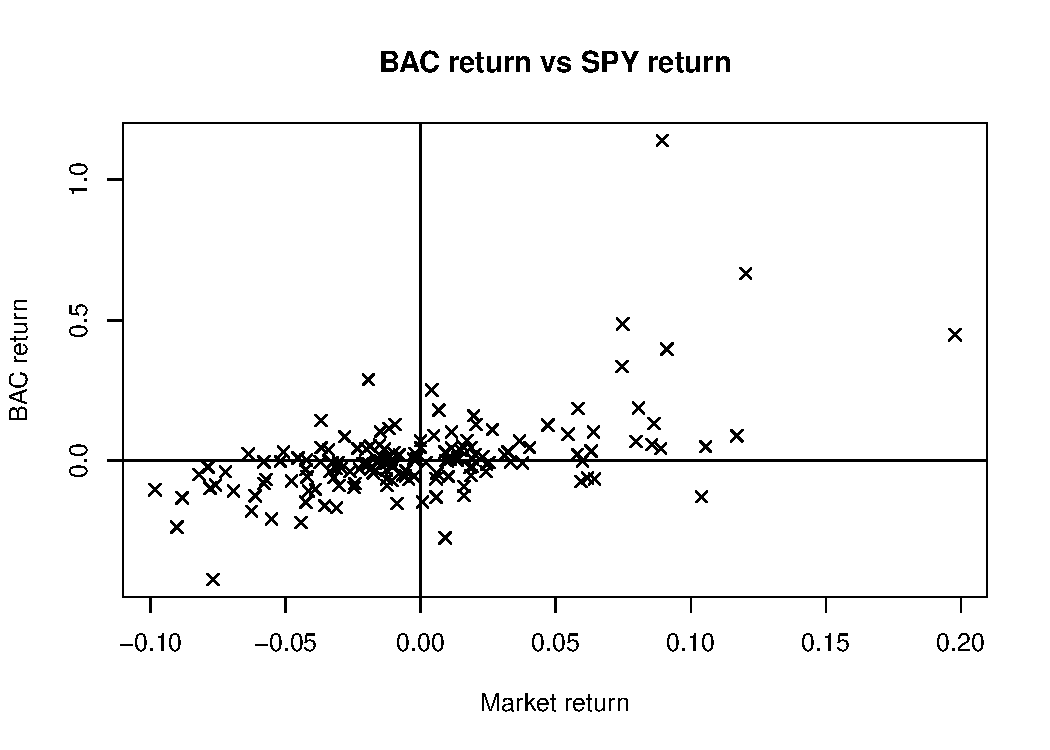
\includegraphics[width=\maxwidth]{figure/Reg1} 

\end{knitrout}


It seems that there is a positive relationship between the two variables.  The aim is to draw a line that will express this relationship between $x$ and $y$.  If we were to draw a line arbitrarily to represent the relationship, it could be denoted

\begin{equation}
y_t = a + bX_t + u_t
\end{equation}

Where, as usual, $a$ would be the intecept on the y axis and $b$ would be the gradient. The gradient $b$ is the relationship between the return on the S\&P 500 and the return on Bank of America.  This is what we want to find out.  The difference between Equation 1 and Equation 2 is that the former is a theoretical model and the latter is an actual equation.   The variable $\varepsilon$ in Equation 1 is the \emph{error term} that represents all the factors that have not been included in the model; $u_t$ is the \emph{residual}  that is the difference between the estimated value of the dependent variable and the actual vale of the dependent variable.  As such, a good model would be one that makes the residuals as small as possible.

If the residuals are just added together the positive and negative numbers will just cancel each other out.  Therefore it is necessary to square the residuals before the addition to create the \emph{Residual Sum of Squares} (RSS).  There are two main ways that the model with the smallest RSS can be identified: the first is to choose an equation, sum the residuals and repeat this process until a minimum has been found; the second , which can be used here but not in all cases, is to use analytical methods to calculate the coefficients that make the minimum.

The first method of trial and error will not be discussed in detail here.  The second method uses calculus to find the minimum value of the RSS.  Using linear algebra for a multiple regression (there is more than one explanatory variable) the solution that will be used by excel, Eviews or any other package is

\begin{align*}
\mathbf{y} =& \mathbf{X \beta} + \mathbf{u}\\
\mathbf{u} =& \mathbf{y} - \mathbf{X\beta}\\
\mathbf{u}' \mathbf{u} =& (\mathbf{X \beta} + \mathbf{u})'(\mathbf{X \beta} + \mathbf{u})\\ 
\end{align*}

Taking derivative and re-arranging (see textbook for proof)
\begin{align*}
\mathbf{\beta} = \mathbf{(X'X)}^{-1}\mathbf{X'y}
\end{align*}

Knowing this is not important for now.  It will be calculated by the software.  It can be useful to understand this analytical solution if you want to know more about the effect of relaxing the OLS assumptions.  You will cover this next year in the Econometrics option. 

\section{OLS results}
Using that formula, the following solution is found. 

The regresion results are shown in Table \ref{tabref:reg}.  The column \emph{Estimate} shows the estimates of the $\beta_0$ and $\beta_1$ from Equation \ref{reg}.  The estimate for $\beta_0$ is 1.83.  This indicates that, on average, the effect of a 1 percent S\&P 500 return is a 1.8\% return for Bank of America. This is the main information that we require. 
% latex table generated in R 3.0.2 by xtable 1.7-1 package
% Wed Dec 25 22:07:07 2013
\begin{table}[ht]\label{tabref:reg}
\centering
\begin{tabular}{rrrrr}
  \hline
 & Estimate & Std. Error & t value & Pr($>$$|$t$|$) \\ 
  \hline
(Intercept) & 0.0130 & 0.0105 & 1.23 & 0.2203 \\ 
  SPY.R & 1.8303 & 0.2240 & 8.17 & 0.0000 \\ 
   \hline
\end{tabular}
\end{table}
\begin{knitrout}
\definecolor{shadecolor}{rgb}{0.969, 0.969, 0.969}\color{fgcolor}

{\centering 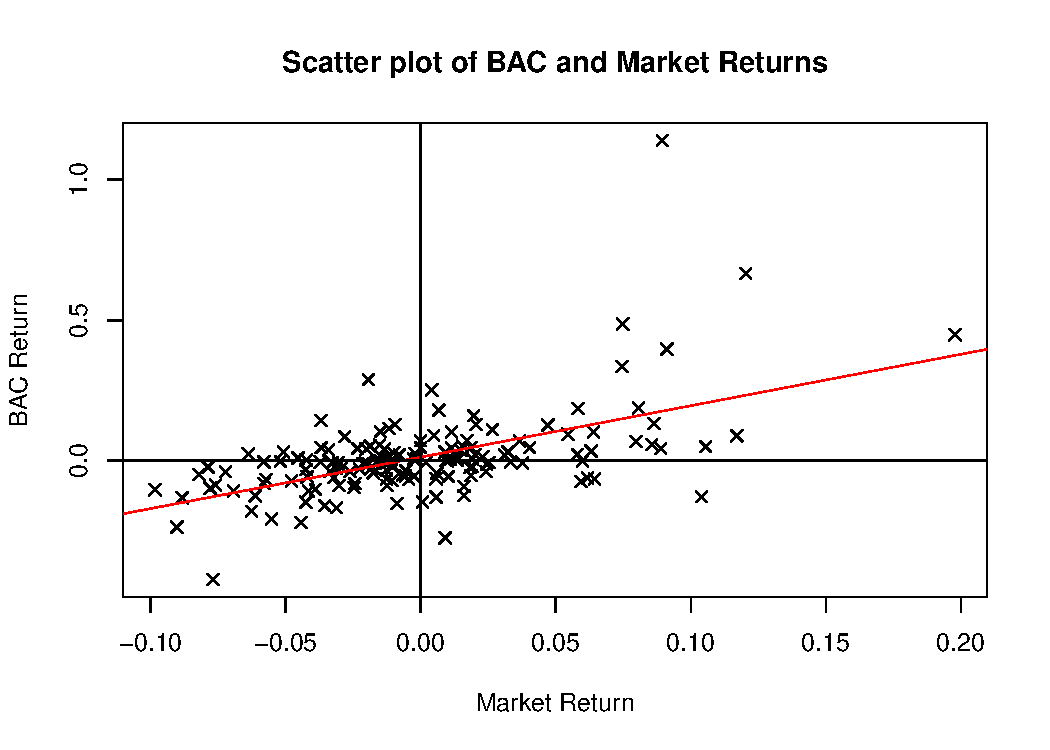
\includegraphics[width=\maxwidth]{figure/Reg2} 

}



\end{knitrout}


The Adjusted $R^2$ is 0.29, therefore nearly 30\% of the BAC returns are explained by the returns of the market.  The \emph{Standard Error} is the estimate of the standard deviation of the estimated coefficient value.  This means that, assuming a normal distribtion, 95\% of the estimates would stand between 2 standard errors of the mean.  Therefore, the 95\% confidence intervals for the $\beta_1$ are 1.39 to 2.27.  This means that under repeated sampling 95\% ofthe estimates of $\beta_1$ should be between these values.  As, if value of $\beta_1$ were really zero, it would be extremly unlikely to get a figure of 1.8\% for this estimate.  The probability of getting this value when it was really zero is in the final column.  This probablity is based on the \emph{t value} which is calculated as
\begin{equation}
t = \frac{\hat{\beta_1} - \beta_n}{SE(\hat{\beta_1})}
\end{equation}
Where $\hat{\beta_1}$ is the estimate of the coefficient (1.83 in our case), $\beta_n$ is the hypothesised value of the coefficient (zero in our case) and $SE(\hat{\beta_1})$ is the estimate of the standard deviation of the estimates of the coeficient (0.224).  Therefore, 
\begin{equation}
t = \frac{1.8 - 0}{0.224} = 8.17
\end{equation}
This is the number of standard deviations that the coefficient is away from the hypothesised value of zero.  If the absolute value of the \emph{t-statistic} is more than 2, there is less than 5 chances in 100 that the coefficient would be see when the actual value was zero.  In that situation we say that the coefficient is \emph{statistically different from zero}. 
Ordinary Least Squares is one way of estimating the model.  Given a number of assumptions, the OLS coefficients are \textbf{BLUE}.  That is the \textbf{B}est \textbf{L}inear \textbf{U}nbiased \textbf{E}stimator.  The assumptions are 
\begin{enumerate}
\item The errors have a zero mean
\item The errors are \emph{independent and identically distributed} (iid)
\begin{itemize}
\item No serial correlation (errors related to each other)
\item Hetroskedasticity (some errors are systematically larger than others)
\end{itemize}
\item Explanatory variables are not related to the error
\item Additionally, assume \emph{normal errors} if we want to use normal assumption to compute \emph{t-tests} of coefficients
\end{enumerate}



\end{document}
